\section{Architekturkonzept}
\label{sec:architekturkonzept}
    Das Framework stellt die Kern-Funktionalität zur Steuerung von implementierten Regeln und Prozessen innerhalb eines 
    Gebäudes, bspw. eines Büroraumes, dar. Mit dem Architekturkonzept wird der grundlegende Aufbau sowie die Funktionalität des Systems erläutert. 
    Potenzielle Erweiterungen und Adaptionen werden im Ausblick (\ref{chap:ausblick}) aufgegriffen.
    \\ 
    \linebreak
    Das System soll in drei Schichten aufgeteilt werden. Die oberste Schicht stellt die Kommunikationsschicht dar, die mittlere 
    die Logik- und Prozessschicht und die unterste die Persistenzschicht. Im Rahmen der Arbeit wird 
    die dritte Schicht nicht detailliert beschrieben, da diese zum aktuellen Zeitpunkt weniger von Interesse ist bzw. für keine weitere Verarbeitung 
    genutzt wird. Die Ausprägung der Schicht wäre dennoch ohne weiteres möglich und wird grob skizziert. Der Abbildung 
    (\ref{fig:schichtenarchitektur}) ist die Aufteilung der Schichtenarchitektur zu entnehmen. In der Darstellung unterscheidet sich die 
    Persistenzschicht farblich von den anderen, da diese im aktuellen Konzept keine konkrete Implementierung erfährt. 
    Das Schaubild zeigt bereits auf dieser Ebene die Trennung der Zuständigkeiten, engl. \textit{seperation of concerns}. 
    Durch die gezielte Abstraktion von Komponenten und Informationen kann die Komplexität 
    eines Systems vereinfacht dargestellt werden. Die Kommunikationsschicht ermöglicht die Anbindung von verschiedensten Kommunikationsprotokollen, die 
    dadurch adaptiert werden können. Im Rahmen des Konzepts wird ausschließlich vom \acs{MQTT}-Protokoll Gebrauch gemacht. 
    Die Logikschicht nimmt alle eingehenden Events der Kommunikationsschicht, die jeweils eine Zustandsänderung hervorrufen können, entgegen 
    und durchläuft den Prozess des Frameworks, um auf die Zustandsänderung die passende Regel auszuführen. Die 
    Persistenzschicht ist für die Speicherung erzeugter Daten verantwortlich, bspw. können bei Zustandsänderungen die Transaktionen 
    als Historie persistiert werden. Ebenso können Informationen gespeichert werden, die anderweitig zur Verfügung stehen würden. Das Vorantreiben der Speicherung 
    von Informationen kann durch den agilen Entwicklungsprozess außerhalb des Thesis-Rahmens erfolgen. 
    \begin{figure}[hbt!]
        \centering
        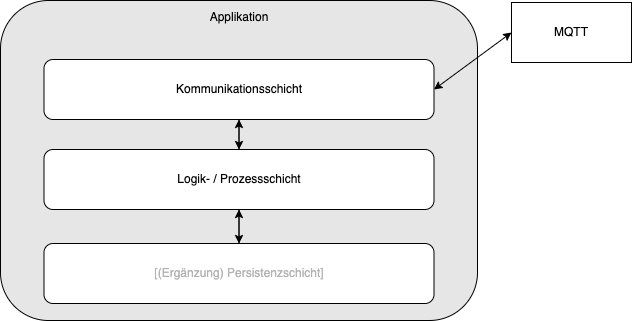
\includegraphics[width=14cm,height=11cm,keepaspectratio]{images/Schichtenarchitektur.png}
        \caption{Schichtenarchitektur}
        \label{fig:schichtenarchitektur}
    \end{figure}
    \\
    %\pagebreak
    Für die Konzeption von wartbarer und erweiterbarer Software wird von den \textit{SOLID}-Prinzipien sowie von nützlichen 
    und für das Framework verwendbaren Programmiermustern Gebrauch gemacht. Diese werden an geeigneter Stelle und auf den Nutzen bezogen erläutert.
    \\
    \linebreak
    Das \textit{SOLID} wurde von Robert C. Martin\footnote{Software Engineer, Lehrer und Autor Robert C. Martin. \url{https://en.wikipedia.org/wiki/Robert_C._Martin} Besucht am 10.07.2022} 
    geprägt und soll zum Design guter objektorientierter Software beitragen. Dadurch soll 
    ein Softwaresystem einer höheren Wartbarkeit unterliegen. Es setzt sich aus fünf Prinzipien zusammen, %\footnote{SOLID Prinzipien. \url{https://blog.cleancoder.com/uncle-bob/2020/10/18/Solid-Relevance.html} Besucht am 10.07.2022}, 
    die wie folgt definiert sind:
    \begin{itemize}
        \item S - Single-Responsibility-Prinzip: „Das Single-Responsibility-Prinzip (SRP; Eine-Verantwortlichkeit-Prinzip; ...) fordert, dass eine Klasse oder ein Modul einen und nur einen \textit{Grund zur Änderung} haben sollte.“ \cite{cleancode2009}
        \item O - Open-Closed-Prinzip: „Module sollten sowohl offen (für Erweiterungen) als auch verschlossen (für Modifikation) sein.“ \cite{ocpmeyer1988}
        \item L - Liskovsches Substitutionsprinzip: „... Sei q(x) eine beweisbare Eigenschaft von Objekten x des Typs T. Dann soll q(y) für Objekte des Typs S wahr sein, wobei S ein Untertyp von T ist.“ \cite{liskov2001behavioral} - Das (Ersetzungs-)Prinzip sagt somit aus, dass eine 
        Subklasse stets die Eigenschaften der Superklasse erfüllt und immer als Objekt der Superklasse anwendbar sein muss. Eine Subklasse darf dadurch erweitert werden, aber 
        keine grundlegende Änderung erfahren. 
        \item I - Interface-Segregation-Prinzip: „Clients sollen nicht dazu gezwungen werden, von Interfaces abzuhängen, die sie nicht verwenden.“ \cite{martin1996interface}
        \item D - Dependency-Inversion-Prinzip: „A. Module hoher Ebenen sollten nicht von Modulen niedriger Ebenen abhängen. Beide sollten von Abstraktionen abhängen. B. Abstraktionen sollten nicht von Details abhängen. Details sollten von Abstraktionen abhängen.“ \cite{martin2003agile}
    \end{itemize}
    Besonders das \textit{Single-Responsibility}- und das \textit{Open-Closed}-Prinzip wurden bei der Konzeption berücksichtigt. 
    Da es sich bei diesem System nicht um eine klassische 
    Webanwendung handelt und keine direkte Kommunikation unter anderem über \acs{REST} \acs{API}s stattfindet, wird ein allgemeines 
    Programmiermuster, wie bspw. das \ac{MVC}\footnote{Architekturmuster für Webapplikationen. \url{https://de.wikipedia.org/wiki/Model_View_Controller} Besucht am 10.07.2022} 
    oder das \ac{MVVM}\footnote{Software-Architekturmuster. \url{https://en.wikipedia.org/wiki/Model–view–viewmodel} Besucht am 10.07.2022 }, nicht 
    in Betracht gezogen. Verwendet werden allgemeine Architekturmuster und -prinzipien, die dazu beitragen, die Software wartbar 
    zu gestalten, die Komplexität einzelner Funktionen zu reduzieren und die Lesbarkeit und Überschaubarkeit zu erhöhen. 
    \pagebreak
    \subsection{Aufbau des Frameworks}
        Nach Veranschaulichung der Schichten-Modellierung werden übergreifend der Komponentenaufbau und die dafür einzusetzenden Architekturmuster aufgegriffen. 
        \\
        Die Konzeptkomponenten (\ref{subsec:conceptcomps}) finden sich im umfassenden Architekturschaubild (siehe Abbildung \ref{fig:patternarchitektur}) wieder. 
        Die Regelstruktur soll die Funktion einer Bedingungsprüfung und der darauffolgenden Aktion vorgeben, damit bestimmte Anhaltspunkte geschaffen werden, die das Framework überprüfen 
        und anwenden kann. Um zu gewährleisten, dass dem Anwender diese Methoden bei Implementierung einer spezifischen Regel zur Verfügung stehen, wird ihm mittels dem 
        \textit{Template Method} Pattern \cite{gamma1995template} (Schablonenmethoden-Entwurfsmusters) ein Leitfaden vorgegeben. Es gehört zu den Verhaltensmustern, engl. behavioral patterns. 
        Ziel des Musters ist die Delegation der konkreten Ausformung einzelner Methoden und Funktionen zu deren Unterklassen. Innerhalb der 
        abstrakten Klasse wird das Skelett des Objektes definiert. Die einzelnen Schritte können so in den darunter liegenden Klassen überschrieben oder ergänzt 
        werden, ohne dass die grundlegende Struktur der übergreifenden Klasse modifiziert werden muss. Die Unterklassen, die konkret die Definition einer Regel ist, sollen 
        unter Verwendung des \textit{Singleton} Patterns \cite{gamma1995singleton} realisiert werden. Das zu den Erzeugungsmustern 
        zugehörige Pattern dient zur 
        Sicherstellung, dass eine Klasse, in dem Fall die einzelne Regel, zur Laufzeit ausschließlich eine einzige Instanz erzeugt und diese global erreichbar ist. 
        Dadurch wird von jeder Regel immer nur ein Objekt erzeugt. 
        \\
        \linebreak
        Ähnlich zum Aufbau des Regelwerks sollen die Komponenten, die reale Gegenstände abbilden, ebenso vom Schablonenmethoden-Entwurfsmuster Gebrauch machen. 
        Unterschied zu der Regel-Schablone ist lediglich die Funktion der Sperrung einer Komponente für weitere Aufgaben. Diese soll bereits in der abstrakten Klasse 
        definiert sein. Konkrete Eigenschaften von Komponenten und konkrete Zustandsattribute können vom Anwender selbst implementiert werden.
        \\
        \linebreak
        Die durch den Anwender implementierte Transformation, die unter anderem basierend auf einem eingehenden \acs{MQTT}-Topic das Zustandsobjekt verändert, soll 
        das {Template Method} Pattern verwenden. Dadurch ist die Struktur der Transformation vorgegeben. Soll ein Transformationsobjekt erzeugt werden, so müssen 
        diesem die notwendigen Parameter übergeben werden. 
        %Innerhalb dieser Schablone sollen alle Attribute vorgegeben werden, die für die Transformation notwendig sind und von dem Softwareentwickler implementiert werden sollen. 
        \\
        \linebreak
        Damit zukünftig weitere Kommunikationsschnittstellen hinzugefügt werden können, soll für die Transformation zusätzlich das 
        \textit{Adapter} Pattern verwendet werden. Dadurch können Events aus unterschiedlichen Services und über mehrere Kommunikationswege 
        entgegengenommen werden, ohne dass die eigentliche Schnittstelle modifiziert werden muss. Das \textit{Adapter} Pattern gehört 
        zu den Strukturmustern und ist wie folgt definiert:
        \\
        „Das \textit{Adapter} Pattern fungiert als Verbinder zwischen zwei inkompatiblen Schnittstellen, die ansonsten nicht direkt verbunden werden können. Ein Adapter umschließt 
        eine vorhandene Klasse mit einer neuen Schnittstelle, sodass sie mit der Schnittstelle des Clients kompatibel wird.“\footnote{Beschreibung des Adapter Entwurfsmusters. \url{https://www.baeldung.com/java-adapter-pattern} Besucht am 10.08.2022} \cite{gamma1995adapter}
        \pagebreak
        \\
        Das Zustandsobjekt ist aus Anwendersicht als ein einfaches \ac{POJO}, ein ganz normales Java Objekt, zu implementieren. Das Framework soll sich um die korrekte Nutzung 
        des Objektes kümmern. 
        \\
        \linebreak
        Der übergreifende Aufbau unter Verwendung von Entwurfsmustern ist folgender Abbildung zu entnehmen:
        \begin{figure}[hbt!]
            \centering
            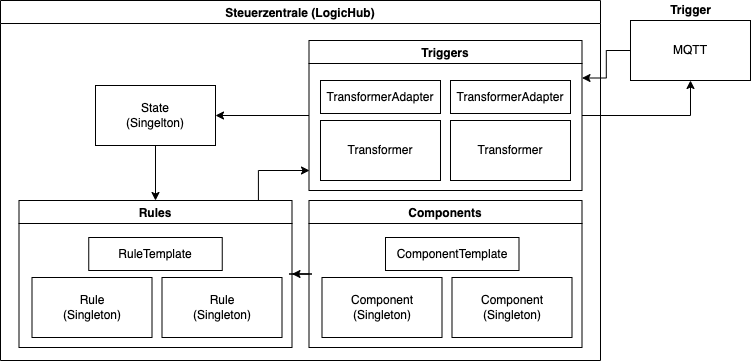
\includegraphics[width=15cm,height=12cm,keepaspectratio]{images/final_architecture_with_patterns.png}
            \caption{Architektur mit verwendeten Entwurfsmustern}
            \label{fig:patternarchitektur}
        \end{figure}
        \\
        Der soeben grob skizzierte Aufbau wird in den folgenden Abschnitten konkretisiert.

    \subsection{Kommunikationsschicht}
    Damit das Framework einer hohen Wartbarkeit und Erweiterbarkeit unterliegt, soll bereits in der Kommunikationsschicht mithilfe 
    des genannten \textit{Adapter} Musters eine Abstraktionsebene geschaffen werden. Diese erleichtert das Adaptieren 
    hinzukommender Kommunikationsschnittstellen, um in Zukunft weitere \acs{IoT}-Protokolle mit dem Framework zu nutzen. 
    Die geplante Struktur kann dem Klassendiagramm in Abbildung (\ref{fig:patternarchitektur}) entnommen werden. 
    Der Client, in dem speziellen Fall der \textit{\acs{MQTT}-Topic-Subscriber}, wird mit einem \textit{Transformationsadapter} versehen. Hierbei wird mit den eingehenden 
    Informationen, die über die Funktion des Subscribers abgegriffen und an das Frameworks übergeben wurden, gearbeitet. 
    Wird eine weitere Kommunikationsschnittstelle hinzugefügt, so muss lediglich ein dafür vorgesehener \textit{Adapter} implementiert werden, der 
    alle für das Framework notwendigen Informationen delegiert. Dadurch bleibt die interne Arbeitsweise des Frameworks unverändert und fördert so die Erweiterbarkeit des 
    Systems.
    \begin{figure}[hbt!]
        \centering
        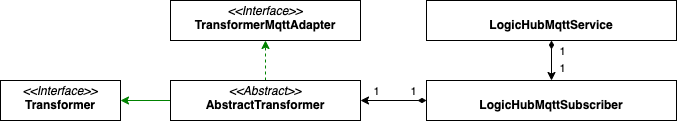
\includegraphics[width=14cm,height=10cm,keepaspectratio]{images/Kommunikationsschicht_final.png}
        \caption{Klassendiagramm der Kommunikationsschicht}
        \label{fig:patternkommunikation}
    \end{figure}
    \pagebreak
    \\
    Der interne Ablauf einer Nachrichtenkonsumierung kann dem Sequenzdiagramm in Abbildung (\ref{fig:kommunikationsequenz}) entnommen werden. Mit der Transformation 
    soll das eingehende \acs{MQTT}-Topic mit den vom Anwender definierten Topics überprüft werden. Gibt es dabei eine Übereinstimmung, soll anhand des Topics die mitgelieferte 
    Nachricht konsumiert und dem jeweiligen Wert im Zustandsraum zugeordnet und dementsprechend überschrieben werden. Mit der Zustandsänderung wird die 
    Prozessschicht des Frameworks aufgerufen, die daraufhin alle dem Framework bekannten Regeln überprüft und die Zutreffenden startet. Der Durchlauf wird im Abschnitt (\ref{subsec:logikschicht}) 
    dargestellt. 
    \begin{figure}[hbt!]
        \centering
        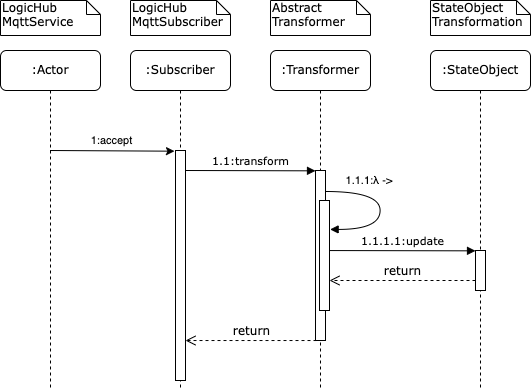
\includegraphics[width=14cm,height=10cm,keepaspectratio]{images/Kommunikationsschicht_Sequenz_Final.png}
        \caption{Sequenzdiagramm zur Kommunikationsschicht}
        \label{fig:kommunikationsequenz}
    \end{figure}

    \subsection{Logik- und Prozessschicht}
    \label{subsec:logikschicht}
    Die Logik- und Prozessschicht wird aktiv, wenn durch eine bestimmte Kommunikationsschnittstelle, im Rahmen der Arbeit ausschließlich durch \acs{MQTT} realisiert, ein eingehendes 
    Event bzw. eine eingehende Nachricht konsumiert und daraufhin das Zustandsobjekt geändert wurde. Die in erster Linie dafür benötigten Objekte sind dem 
    Klassendiagramm (\ref{fig:patternlogik}) zu entnehmen. Die an zentraler Stelle stehende Klasse des \textit{LogicHubState} soll die Koordination 
    der Zustandsänderung sowie das nachträgliche Prüfen der Regelbedingungen und das Ausführen des Regelprozesses übernehmen. 
    \\
    Die \textit{LogicHubState} Klasse muss eine \textit{setState}-Methode enthalten, die die Schritte der Zustandsänderung und die des Kopiervorgangs des Zustandsobjektes beinhaltet. 
    In der vorgesehenen Funktion wird anschließend mit der Kopie des Zustandsraumes und der hierin immanierten Änderung gearbeitet, indem daraufhin das Regelwerk durchlaufen wird und die Bedingungen 
    der darin enthaltenen Regel überprüft werden. Durch die Verwendung der Kopie zum Durchlaufen der zutreffenden Regelprozesse entsteht keine Inkonsistenz des eigentlichen Zustandsraums.  
    Somit wird verhindert, dass eine Zustandsänderung durch eine Regel das repräsentative Zustandsobjekt direkt manipuliert. Dadurch können Regelprozesse asynchron abgearbeitet werden 
    und so mehrere Zustandsänderungen erfolgen. Zusätzlich wird der Kopiervorgang gesperrt, sodass keine Inkonsistenz des Zustandes durch gleichzeitig hereinkommende Änderungen entsteht. 
    \begin{figure}[hbt!]
        \centering
        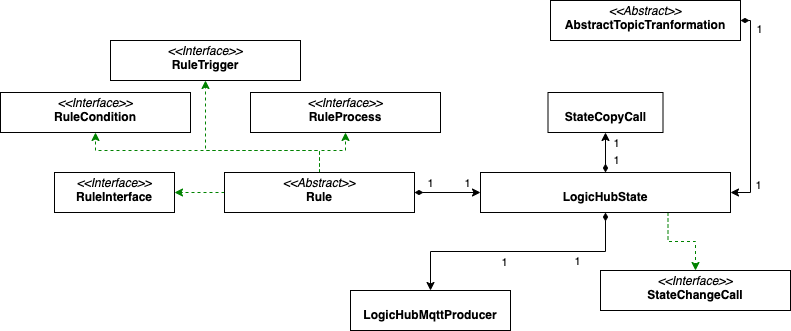
\includegraphics[width=14cm,height=10cm,keepaspectratio]{images/Logikschicht_final.png}
        \caption{Klassendiagramm zur Logik- und Prozessschicht}
        \label{fig:patternlogik}
    \end{figure}
    \\
    Der initiale Ablauf von der Zustandsänderung bis hin zur Prüfung der Regelbedingung über die Erstellung einer Kopie sowie das anschließende Durchführen kann dem folgenden Sequenzdiagramm entnommen werden. 
    \\
    \pagebreak
    \begin{figure}[hbt!]
        \centering
        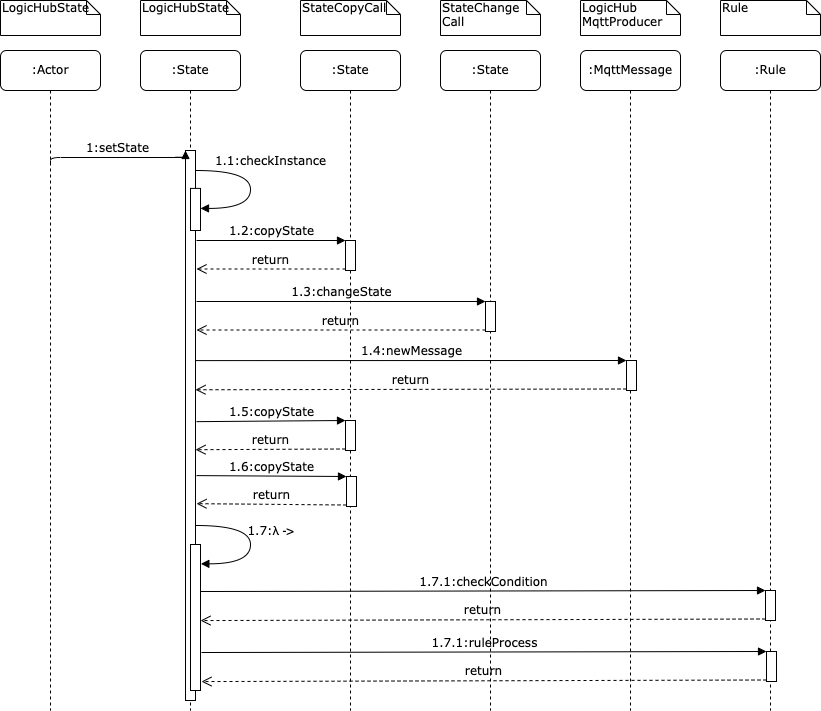
\includegraphics[width=14cm,height=14cm,keepaspectratio]{images/Logikschicht_Sequenz_final.png}
        \caption{Sequenzdiagramm zur Logikschicht}
        \label{fig:logiksequenz}
    \end{figure}
    \\
    %\linebreak
    Das Diagramm (\ref{fig:logiksequenz}) beinhaltet ebenso die inverse Transformation (\ref{subsec:inverseTransformation}). Mithilfe dieser sollen erneute 
    Zustandsänderungen, die der Anwender durch eine Regel definiert, stattfinden, bspw. zur Veröffentlichung von Steuerbefehlen über eine \acs{MQTT}-Nachricht. %von Nachrichten über \acs{MQTT}, um Steuerbefehle die erzielt wird, wenn durch eine Regel eine erneute Zustandsänderung stattfindet, die bspw. Befehle über \acs{MQTT} 
    %veröffentlicht, um Komponenten steuern zu können. 
    Auf die konkrete Umsetzung der soeben architektonisch beschriebenen Komponenten wird im folgenden Kapitel (siehe Umsetzung \ref{chap:umsetzung}) 
    eingegangen. 
    \\
    Die Ausprägung der Persistenzschicht wurde im Rahmen dieser Arbeit nicht weiter detailliert aufgezeigt, da zum aktuellen Zeitpunkt 
    kein Bedarf an der Speicherung von Historien oder Zustandsänderungen besteht. Dennoch wird an dieser Stelle erwähnt, dass die Einbindung einer 
    Datenbank sowie die Modellierung der Datenobjekte und deren Speicherung ohne weiteres möglich ist. 
\\
\linebreak
Für die Generierung mehrerer konkurrierender Sichten wurden die Diagramme, darunter Klassen- und Sequenzdiagramme 
(siehe \ref{fig:patternkommunikation}, \ref{fig:kommunikationsequenz}, \ref{fig:patternlogik} \& \ref{fig:logiksequenz}) 
unter Verwendung des \textit{4+1 Sichtenmodells} von Philippe Kruchten \cite{Kruchten1995}, erstellt. 
Die Beschreibung der Szenarien fand bereits in der Anforderungsanalyse (siehe \ref{subsec:checkin} \& \ref{subsec:evacuation}) statt. 
Nach Beendigung der Konzeption wird im folgenden Kapitel die Umsetzung des Konzeptes und die 
Implementierung des Prototypen vertieft. 
